\documentclass{article}\usepackage[]{graphicx}\usepackage[]{xcolor}
% maxwidth is the original width if it is less than linewidth
% otherwise use linewidth (to make sure the graphics do not exceed the margin)
\makeatletter
\def\maxwidth{ %
  \ifdim\Gin@nat@width>\linewidth
    \linewidth
  \else
    \Gin@nat@width
  \fi
}
\makeatother

\definecolor{fgcolor}{rgb}{0.345, 0.345, 0.345}
\newcommand{\hlnum}[1]{\textcolor[rgb]{0.686,0.059,0.569}{#1}}%
\newcommand{\hlsng}[1]{\textcolor[rgb]{0.192,0.494,0.8}{#1}}%
\newcommand{\hlcom}[1]{\textcolor[rgb]{0.678,0.584,0.686}{\textit{#1}}}%
\newcommand{\hlopt}[1]{\textcolor[rgb]{0,0,0}{#1}}%
\newcommand{\hldef}[1]{\textcolor[rgb]{0.345,0.345,0.345}{#1}}%
\newcommand{\hlkwa}[1]{\textcolor[rgb]{0.161,0.373,0.58}{\textbf{#1}}}%
\newcommand{\hlkwb}[1]{\textcolor[rgb]{0.69,0.353,0.396}{#1}}%
\newcommand{\hlkwc}[1]{\textcolor[rgb]{0.333,0.667,0.333}{#1}}%
\newcommand{\hlkwd}[1]{\textcolor[rgb]{0.737,0.353,0.396}{\textbf{#1}}}%
\let\hlipl\hlkwb

\usepackage{framed}
\makeatletter
\newenvironment{kframe}{%
 \def\at@end@of@kframe{}%
 \ifinner\ifhmode%
  \def\at@end@of@kframe{\end{minipage}}%
  \begin{minipage}{\columnwidth}%
 \fi\fi%
 \def\FrameCommand##1{\hskip\@totalleftmargin \hskip-\fboxsep
 \colorbox{shadecolor}{##1}\hskip-\fboxsep
     % There is no \\@totalrightmargin, so:
     \hskip-\linewidth \hskip-\@totalleftmargin \hskip\columnwidth}%
 \MakeFramed {\advance\hsize-\width
   \@totalleftmargin\z@ \linewidth\hsize
   \@setminipage}}%
 {\par\unskip\endMakeFramed%
 \at@end@of@kframe}
\makeatother

\definecolor{shadecolor}{rgb}{.97, .97, .97}
\definecolor{messagecolor}{rgb}{0, 0, 0}
\definecolor{warningcolor}{rgb}{1, 0, 1}
\definecolor{errorcolor}{rgb}{1, 0, 0}
\newenvironment{knitrout}{}{} % an empty environment to be redefined in TeX

\usepackage{alltt}
\usepackage{amsmath} %This allows me to use the align functionality.
                     %If you find yourself trying to replicate
                     %something you found online, ensure you're
                     %loading the necessary packages!
\usepackage{amsfonts}%Math font
\usepackage{graphicx}%For including graphics
\usepackage{hyperref}%For Hyperlinks
\usepackage[shortlabels]{enumitem}% For enumerated lists with labels specified
                                  % We had to run tlmgr_install("enumitem") in R
\hypersetup{colorlinks = true,citecolor=black} %set citations to have black (not green) color
\usepackage{natbib}        %For the bibliography
\setlength{\bibsep}{0pt plus 0.3ex}
\bibliographystyle{apalike}%For the bibliography
\usepackage[margin=0.50in]{geometry}
\usepackage{float}
\usepackage{multicol}

%fix for figures
\usepackage{caption}
\newenvironment{Figure}
  {\par\medskip\noindent\minipage{\linewidth}}
  {\endminipage\par\medskip}
\IfFileExists{upquote.sty}{\usepackage{upquote}}{}
\begin{document}

\vspace{-1in}
\title{Lab 10 -- MATH 240 -- Computational Statistics}

\author{
  Andrew Li \\
  Colgate University  \\
  Math department  \\
  {\tt ali@colgate.edu}
}

\date{04/08/2025}

\maketitle

\begin{multicols}{2}
%\raggedcolumns % If your spacing gets messed up try uncommenting 
                % this line
\begin{abstract}
In this lab, we conducted a simulation study and explored resampling to learn how they can be used to model real world data. Then, we explored what the margin of error of a value can mean and what variables have an impact on it. 
\end{abstract}

\noindent \textbf{Keywords:} Margin of error, resampling, sample size

\section{Introduction}
Gallup polls described their polling process in a document called ``\textit{How are Polls Conducted}" and made several claims about their margin of error, one being doubling sampling size from 1004 to 2000 halves their MOE from 4\% to 2\%. The margin of error helps us understand the variation of our sample proportion as an estimate of the population proportion, and we can estimate the MOE by assuming the population proportion to create a simulated study. However, there are times when the population proportion is unknown, and resampling makes it possible to gather information about the population by using the original sample.

To see what other factors may affect the margin on error besides sampling size, we calculated the margin of error that provides 95\% confidence interval over different sample sizes and proportions. Then, we found the Wilson MOE formula to get more information. 

% \begin{Figure}
% 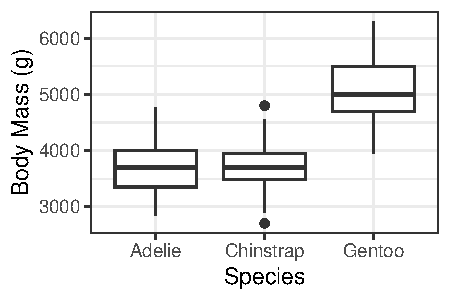
\includegraphics{penguins.pdf}
% \captionof{figure}{This is a figure!} \label{fig:penguins}
% \end{Figure}

\begin{Figure}
% latex table generated in R 4.3.3 by xtable 1.8-4 package
% Tue Apr  1 07:26:31 2025
%\begin{table}[H]% YOU NEED TO REPLACE THIS WITH FIGURE
\centering
\begin{tabular}{lrrrr}
  \hline
species & Mean & Median & SD & IQR \\ 
  \hline
Adelie & 3700.66 & 3700.00 & 458.57 & 650.00 \\ 
  Chinstrap & 3733.09 & 3700.00 & 384.34 & 462.50 \\ 
  Gentoo & 5076.02 & 5000.00 & 504.12 & 800.00 \\ 
   \hline
\end{tabular}
%\caption{This is a table.} % YOU NEED TO CHANGE THIS TO captionof
\captionof{table}{This is a table.} 
\label{tab:penguins}
%\end{table} % YOU NEED TO REPLACE THIS WITH FIGURE
\end{Figure}

\section{Methods}
First, we tested the claim if increasing sample sizes from 1000 to 2000 would reduce the MOE. With the \texttt{rbinom()} function from the \texttt{stats} \citep{stats} package, we created 10000 polls of size 1004 with an assumed population proportion of 0.39 and plotted a histogram of the sampling distribution using \texttt{tidyverse} \citep{tidyverse} package. Then, we repeated the process with polls of size 2008 to measure the difference in moe. 

Using the Gallup poll from February 2025, we have a sample size of 1004 from people across the 50 states and have a sample proportion of 39\% for the people who were satisfied with global standing of the US. Knowing this, we represented that sample with a numeric vector of size 1004. 39\% of the entries were 1's to stand for the people who were satisified and the rest were 0's for those who were dissatisified or neutral. Those two groups can be put together as the focus on is on the 39\%. 

By resampling the data 10000 times with the basic \texttt{R} function \texttt{sample()}, we can approximate the sampling distribution for the sample proportion without knowing the actual population proportion. 

\section{Results}
The histograms of the polls are shown below. They both follow a relatively normal distribution with little skewness, but the sampling distribution for the smaller sample size in Figure \ref{plot1} has a larger variability compared to the Figure \ref{plot2}. This matches with the calculated margin of errors as the polls with sample size of 1004 had a MOE of 0.0309 (approximately 3.1\%), and the polls with sample size of 2008 had a MOE of 0.0211 (approximately 2.1 \%). The MOE for sample size 1004 is within the projected 4\% and while the 2.1\% is slightly more than the Gallup polls statement of within 2\% MOE, it is still very close for the polls of sample size 2008. 

\newpage

\begin{figure}
\begin{center}
\begin{knitrout}
\definecolor{shadecolor}{rgb}{0.969, 0.969, 0.969}\color{fgcolor}
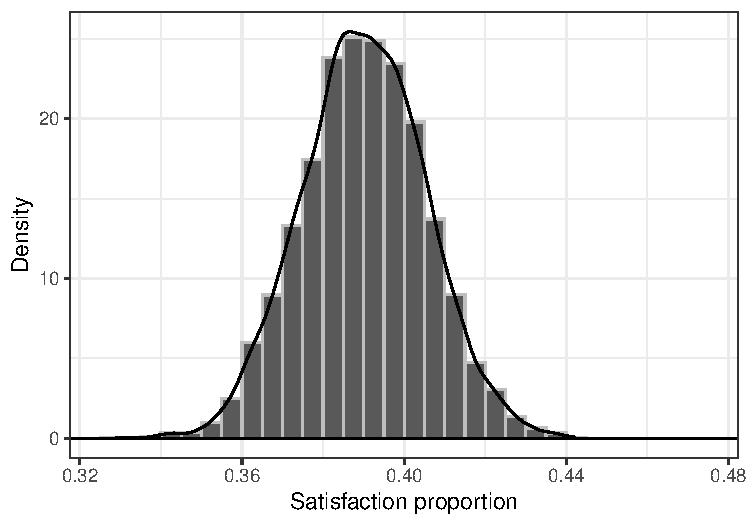
\includegraphics[width=\maxwidth]{figure/unnamed-chunk-2-1} 
\end{knitrout}
\caption{10000 polls with p= 0.39 and n = 1004}
\label{plot1} 
\end{center}
\end{figure}


\begin{figure}[H]
\begin{center}
\begin{knitrout}
\definecolor{shadecolor}{rgb}{0.969, 0.969, 0.969}\color{fgcolor}
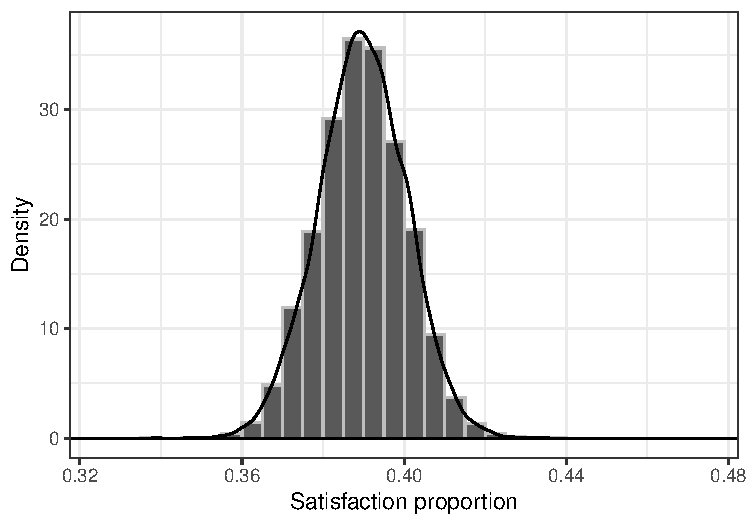
\includegraphics[width=\maxwidth]{figure/unnamed-chunk-3-1} 
\end{knitrout}
\caption{10000 polls with p= 0.39 and n = 2008}
\label{plot2} 
\end{center}
\end{figure}


The histogram of the resampled polls is shown in Figure \ref{plot3}. It follows a relatively normal distribution and looks closer shape to the Figure \ref{plot1}. The MOE is 0.0303 (approximately 3\%), which matches the Gallup's statement that their February 2025 poll was within 4\% MOE. 



\begin{figure}[H]
\begin{center}
\begin{knitrout}
\definecolor{shadecolor}{rgb}{0.969, 0.969, 0.969}\color{fgcolor}
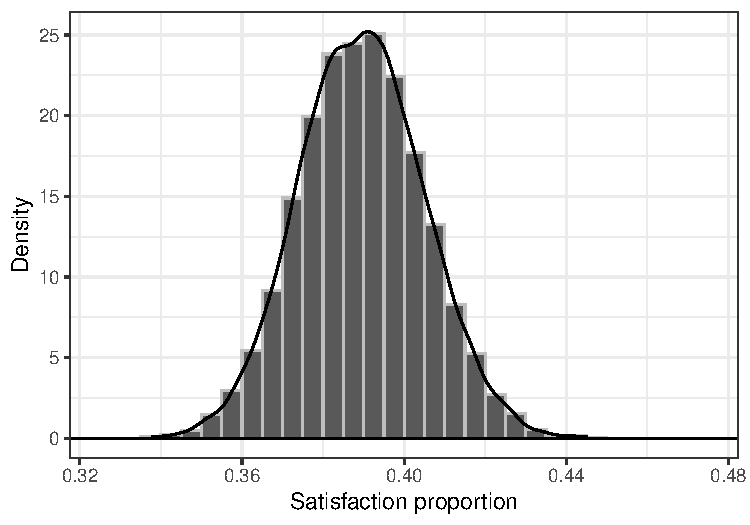
\includegraphics[width=\maxwidth]{figure/unnamed-chunk-4-1} 
\end{knitrout}
\caption{10000 polls from resampling orginal sample}
\label{plot3} 
\end{center}
\end{figure}


We finally look at the effects of the sample size and proportions on MOEs. Figure \ref{plot4} is the estimated MOEs and Figure \ref{plot5} is the Wilson MOEs. As sample size increases, the MOEs decreases. However, the MOE also decreases as proportion gets closer to 1 or 0 because the formula for MOE uses p(1-p),  which becomes incredibly small when dealing with sample proportions close to the maximum or mimimum values. 




\begin{figure}[H]
\begin{center}

\caption{MOE when comparing n vs p}
\label{plot4} 
\end{center}
\end{figure}

\begin{figure}[H]
\begin{center}
\begin{knitrout}
\definecolor{shadecolor}{rgb}{0.969, 0.969, 0.969}\color{fgcolor}
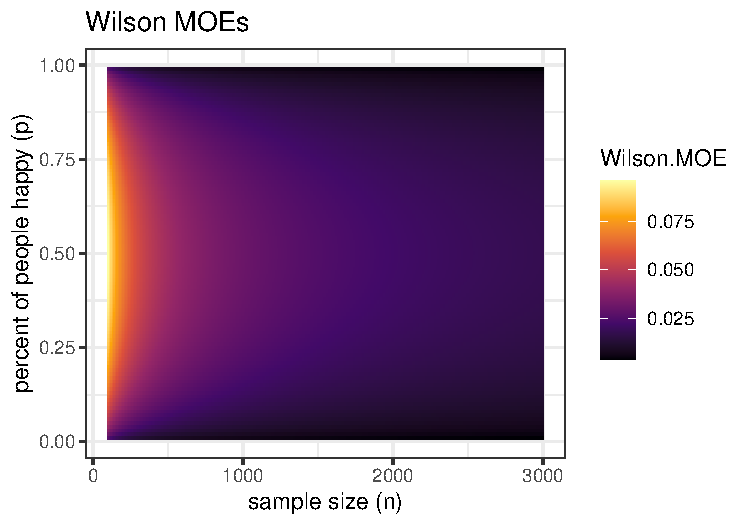
\includegraphics[width=\maxwidth]{figure/unnamed-chunk-6-1} 
\end{knitrout}
\caption{Wilson MOE when comparing n vs p}
\label{plot5} 
\end{center}
\end{figure}

\section{Discussion}
 After looking at the data, there is a decrease for increasing sample sizes, but the margin of error only gets reduced by 1\% for doubling the sample size from 1000 to 2000. Depending how long it takes to conduct these polls or the cost of them, it might not be worthwhile to upscale them. Bigger sample sizes does reduce the margin of error, but so does sample proportion close to 1 and 0.

%%%%%%%%%%%%%%%%%%%%%%%%%%%%%%%%%%%%%%%%%%%%%%%%%%%%%%%%%%%%%%%%%%%%%%%%%%%%%%%%
% Bibliography
%%%%%%%%%%%%%%%%%%%%%%%%%%%%%%%%%%%%%%%%%%%%%%%%%%%%%%%%%%%%%%%%%%%%%%%%%%%%%%%%
\vspace{2em}

\begin{tiny}
\bibliography{bib}
\end{tiny}
\end{multicols}

%%%%%%%%%%%%%%%%%%%%%%%%%%%%%%%%%%%%%%%%%%%%%%%%%%%%%%%%%%%%%%%%%%%%%%%%%%%%%%%%
% Appendix
%%%%%%%%%%%%%%%%%%%%%%%%%%%%%%%%%%%%%%%%%%%%%%%%%%%%%%%%%%%%%%%%%%%%%%%%%%%%%%%%


\end{document}
